% !TEX encoding = UTF-8 Unicode
\documentclass[a4paper]{article}

\usepackage{color}
\usepackage{url}
\usepackage[T2A]{fontenc} % enable Cyrillic fonts
\usepackage[utf8]{inputenc} % make weird characters work
\usepackage{graphicx}
\usepackage{float}

\usepackage[english,serbian]{babel}

\usepackage[unicode]{hyperref}
\hypersetup{colorlinks,citecolor=green,filecolor=green,linkcolor=blue,urlcolor=blue}

\usepackage{listings}

\newtheorem{primer}{Primer}[section]

\definecolor{mygreen}{rgb}{0,0.6,0}
\definecolor{mygray}{rgb}{0.5,0.5,0.5}
\definecolor{mymauve}{rgb}{0.58,0,0.82}

\lstset{ 
  backgroundcolor=\color{white},   % choose the background color; you must add \usepackage{color} or \usepackage{xcolor}; should come as last argument
  basicstyle=\scriptsize\ttfamily,        % the size of the fonts that are used for the code
  breakatwhitespace=false,         % sets if automatic breaks should only happen at whitespace
  breaklines=true,                 % sets automatic line breaking
  captionpos=b,                    % sets the caption-position to bottom
  commentstyle=\color{mygreen},    % comment style
  deletekeywords={...},            % if you want to delete keywords from the given language
  escapeinside={\%*}{*)},          % if you want to add LaTeX within your code
  extendedchars=true,              % lets you use non-ASCII characters; for 8-bits encodings only, does not work with UTF-8
  firstnumber=1000,                % start line enumeration with line 1000
  frame=single,	                   % adds a frame around the code
  keepspaces=true,                 % keeps spaces in text, useful for keeping indentation of code (possibly needs columns=flexible)
  keywordstyle=\color{blue},       % keyword style
  language=Python,                 % the language of the code
  morekeywords={*,...},            % if you want to add more keywords to the set
  numbers=left,                    % where to put the line-numbers; possible values are (none, left, right)
  numbersep=5pt,                   % how far the line-numbers are from the code
  numberstyle=\tiny\color{mygray}, % the style that is used for the line-numbers
  rulecolor=\color{black},         % if not set, the frame-color may be changed on line-breaks within not-black text (e.g. comments (green here))
  showspaces=false,                % show spaces everywhere adding particular underscores; it overrides 'showstringspaces'
  showstringspaces=false,          % underline spaces within strings only
  showtabs=false,                  % show tabs within strings adding particular underscores
  stepnumber=2,                    % the step between two line-numbers. If it's 1, each line will be numbered
  stringstyle=\color{mymauve},     % string literal style
  tabsize=2,	                   % sets default tabsize to 2 spaces
  title=\lstname                   % show the filename of files included with \lstinputlisting; also try caption instead of title
}

\begin{document}

\title{Klasifikacija podataka o kreditnim karticama\\ \small{Seminarski rad u okviru kursa\\Istraživanje podataka\\ Matematički fakultet}}

\author{Tamara Radovanović 430/2016}

%\date{9.~april 2015.}

\maketitle

\abstract{
U okviru ovog rada biće prikazane metode za klasifikaciju koje su učene na kursu Istraživanje podataka i njihova primena na skupu podataka o kreditnim karicama.}

\tableofcontents

\newpage

\section{Uvod}
\label{sec:uvod}

Za istraživanje korišćen je skup podataka o klijentima banke. Ovaj skup podataka sadrži informacije o podrazumevanim plaćanjima, demografskim faktorima, kreditnim podacima, istoriji plaćaanja i računima klijenata kreditnih kartica na Tajvanu od aprila 2005. do septembra 2005. godine.

Baza sadrži 7000 instanci sa po 25 atributa. Ti atributi su:
\begin{itemize}
	\item \textbf{ID:} identifikacija klijenta
	\item \textbf{LIMIT\_BAL:} Količina dodeljenog kredita
	\item \textbf{EDUCATION:} edukacija  (1=graduate school, 2=university, 3=high school, 4=other, 5=unknown)
	\item \textbf{SEX:} Pol (1=male, 2=female)
	\item \textbf{MARRIAGE:} Bračni status (1= married, 2=single, 3=other)
	\item \textbf{AGE:} Starost u godinama 
	\item \textbf{PAY\_0-PAY\_6:} Status otplate u periodu od aprila do septembra 2005. godine
	\item \textbf{BILL\_AMT1-BILL\_AMT6:} Stanje računa od aprila do septambra 2005. godine
	\item \textbf{PAY\_AMT1-PAY\_AMT6:} Količina prethodne upalate od aprila do septambra 2005. godine
	\item \textbf{default.payment.next.month:} Redovna uplata (1=Yes, 0=No)
\end{itemize}

Nad ovim podacima su primenjeni algotirmi za klasterovanje. Prikazani su rezultati, njihovo međusobno uporođivanje.

\section{Priprema podataka}
Podaci sadže informaciju o jednistenoj identifikaciji klijenta, koji ne utiču na verovatnoću da klijent vrati kredit. Iz tog razloga podaci o ID se ne uzimaju u razmatranje.

Podaci o BILL AMT i PAY AMT sadrže kontinualne podatke i za njih treba proveriti da li posotje ekstremne vrednosti i elementi van granice.Instance koje sadrže ekstremne vrednosti nisu uzete u razmatranje, a onima koje sadže elemente van granice su te vrednosti zamenjene najbližom vrednošću koja se ne smatra elementom van granice.  Na slikama \ref{fig:BILL_AMT_pre} i \ref{fig:BILL_AMT_nakon} se mogu videti vrednosti podataka pre i posle obrade ekstremnih vrednosti.

Atribut SEX sadrži vrednosti 1 i 2 i one su promenjene u "male" odnosno "female" radi bolje preglednosti. Kod EDUCATION vrednosti 1-3 su zamenjene redom sa "graduate school", "university" i "high school", a sve ostale sa "other". Kod atributa MARRIAGE urađeno je slično, vrednosti 1 i 2 su zamenjene sa "married" i \char`\"single", a ostale sa "other".
\begin{figure}[h!]
\begin{center}
    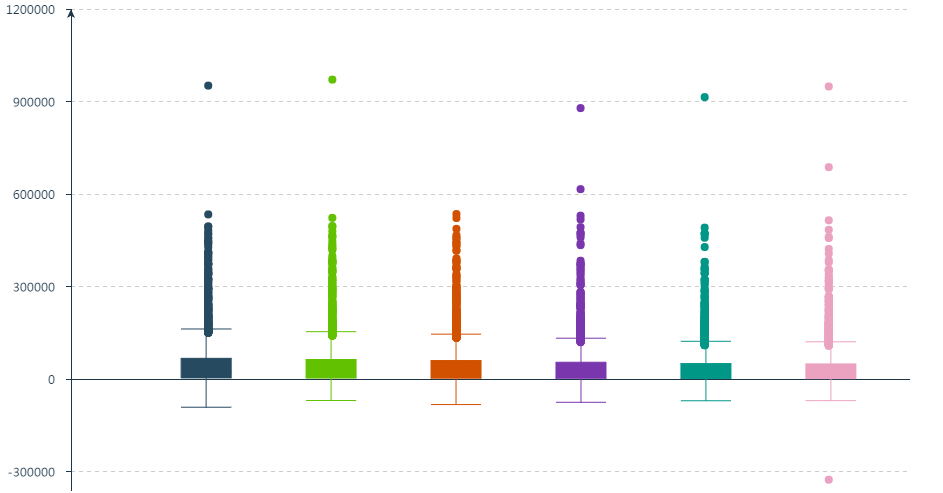
\includegraphics[scale=0.5]{bill_amt.png}
    \caption{Vrednosti BILL\_AMT atibuta pre uklanjanja ektremnih vrednosti}
    \label{fig:BILL_AMT_pre}
\end{center}
\end{figure}


\begin{figure}[h!]
\begin{center}
    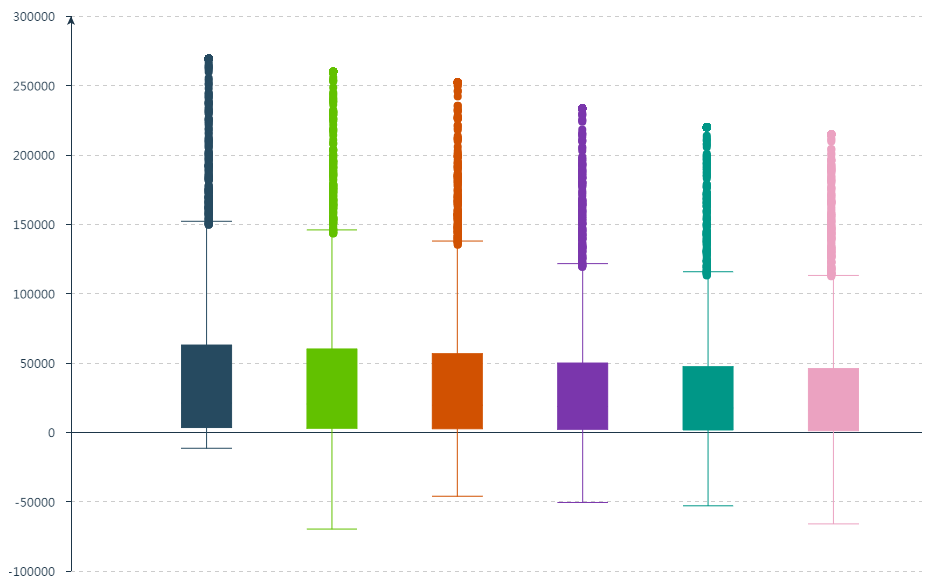
\includegraphics[scale=0.5]{bill_amt_coerce.png}
    \caption{Vrednosti BILL\_AMT atribura nakon uklanjanja ektremnih vrednosti}
    \label{fig:BILL_AMT_nakon}
\end{center}
\end{figure}


\clearpage
\section{C5.0}	
\label{sec:c5.0}

Klasifikaicioni algoritam C5.0 pravi drvo odlučivanja na osnovu koga se određuje kojoj klasi instanca treba da pripada.

Primenom C5.0 algoritma se dobija model čija se uspešnost može videti u tebeli \ref{tab:tabelaC5} kao i mtrica konfuzije u tabeli \ref{tab:tabelaC5matricaKonfuzije}.

\begin{table}[h!]
\begin{center}
\caption{Uspešnost C5.0. algoritme}
\begin{tabular}{|c|l|r|c|c|} \hline
& Trening& & Test & \\ \hline
Tacni &12.278 &82.5\% &12.324 &81.52\% \\ \hline
Netacni &2.605 &17.5\% &2.793 &18.48\% \\ \hline
\end{tabular}
\label{tab:tabelaC5}
\end{center}
\end{table}

\begin{table}[h!]
\begin{center}
\caption{Matrica konfuzije za C5.0 algoritam za test skup}
\begin{tabular}{|c|l|l|l|l|} \hline
& No& Yes \\ \hline
No &TN 11.255 &FP 444 \\ \hline
Yes &FN 2.349 &TP 1.069  \\ \hline
\end{tabular}
\label{tab:tabelaC5matricaKonfuzije}
\end{center}
\end{table}

Iz matrice konfuzije možemo ustanoviti na koji nači model raporedjuje insnce po klasama:
\begin{itemize}
    \item TPR= 0.312756 (stopa stvarno pozitvnih)
    \item TNR= 0.962048 (stopa stvarno negativnih)
    \item FPR= 0.037952 (stopa lažno pozitvnih)
    \item FNR= 0.687244 (stopa lažno negativnih)
\end{itemize}

Na osnovu stope stvarno negativnih i stvarno pozitivnih vidimo da je model skloniji da dobro klasifikuje instance iz "No" klase. Ovakvi rezultati su očekivani jer u korišćenom skupu preovlađuju instance koje pripadaju klasi "No", pa je potrebno uraditi balansiranje klasa. Na slici \ref{fig:balanca} se može videti odnos između klasa pre i posle balansiranja.


\begin{figure}[h!]
\begin{center}
    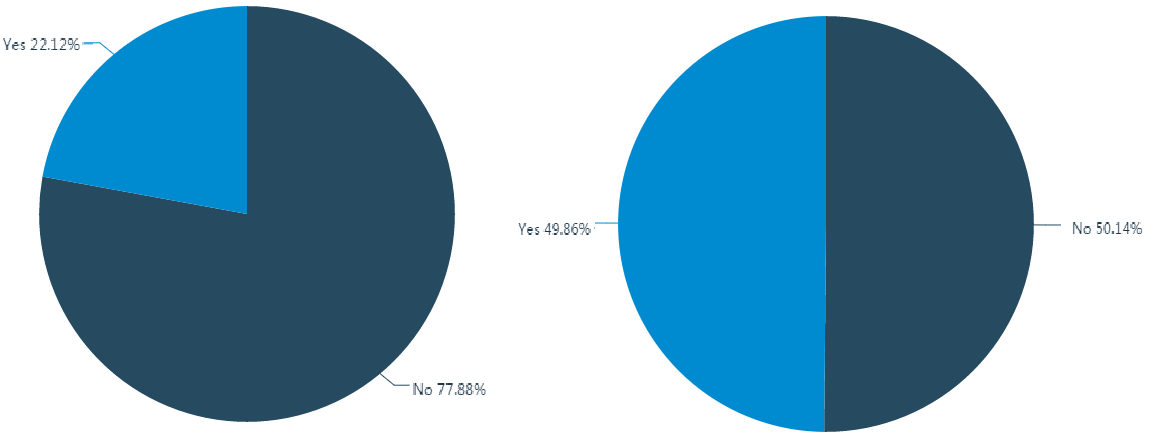
\includegraphics[scale=0.15]{balance.png}
    \caption{Odnos klasa pre i posle balansiranja}
    \label{fig:balanca}
\end{center}
\end{figure}


Za balansiranje klasa se mogu koristit dve tehnike. Prva je da se iz veće klasa izbaci deo instanci, tako da broj istanci ostane isti u obe klasa, dok druga podazumeva da se instance iz manje klase umnože nakon čega će klase biti balansirane.
Primenjene su obe tehnike nad podacima i zatim algoritam C5.0, rezultati se mogu videti u tabelama 
\ref{tab:tabelaC5Balans1} i \ref{tab:tabelaC5Balans2}. Matrica konfuzije koja je dobijen korišćenjem balansiranih podataka se može videti u tabeli \ref{tab:tabelaC5matricaKonfuzijeBalans}, a mere za ocenu modela su sledeće:

\begin{itemize}
    \item TPR= 0.822608 (stopa stvarno pozitvnih)
    \item TNR= 0.801415 (stopa stvarno negativnih)
    \item FPR= 0.198585 (stopa lažno pozitvnih)
    \item FNR= 0.177392 (stopa lažno negativnih)
\end{itemize}
Model napravljen pomoću blansiranih podataka nije nakoljen ni jednoj klasi i daje ujednačene razulate.

\begin{table}[h!]
\begin{center}
\caption{C5.0 algoritam nad balansiranim podacima sa smanjenim brojem instanci "No" klase.}
\begin{tabular}{|c|l|r|c|c|} \hline
& Trening& & Test & \\ \hline
Tacni &22,382&68.69\%&6,447&69.12\%\\ \hline
Netacni&12,204 &31.31\%&2,880&30.88\%\\ \hline
\end{tabular}
\label{tab:tabelaC5Balans1}
\end{center}
\end{table}

\begin{table}[h!]
\begin{center}
\caption{C5.0 algoritam nad balansiranim podacima sa povećanim brojem instanci "Yes" klase.}
\begin{tabular}{|l|l|l|l|l|} \hline
& Trening& & Test & \\ \hline
Tacni &26,386&80,97\%&7,593&81,41\%\\ \hline
Netacni&6,201 &19.03\%&1.734&18.59\%\\ \hline
\end{tabular}
\label{tab:tabelaC5Balans2}
\end{center}
\end{table}

\begin{table}[h!]
\begin{center}
\caption{Matrica konfuzije za C5.0 algoritam nakon balansiranja za test skup}
\begin{tabular}{|c|l|r|c|c|} \hline
& No& Yes \\ \hline
No &TN 3.737 &FP 926 \\ \hline
Yes &FN 827 &TP 3835 \\ \hline
\end{tabular}
\label{tab:tabelaC5matricaKonfuzijeBalans}
\end{center}
\end{table}

Nakon umnožavanja instanci klase "Yes" algoritam daje značajno bolje rezultate jer ne dolazi do gubitka informacija, pa će ova tehnika biti korišćena u ovom algoritmu, kao i u narednim algoritmima.

C5.0 algoritam pruža mogućnost boosting metode, kao i unkrsne validacije. Primenom ovih metoda uspešnost algoritma se povećava. Rezultati se mogu naći u tabeli \ref{tab:tabelaC5Boosting}. Preciznost algotitma kao i mera nečistoće računata preko Ginijevog indeksa se može videti u tablei \ref{tab:tabelaC5Bosting Preciznost}.

\begin{table}[h!]
\begin{center}
\caption{C5.0 algoritam korišćenjem boosting metode i unakrsne validacija.}
\begin{tabular}{|l|l|l|l|l|} \hline
& Trening& & Test & \\ \hline
Tacni &29,845&91,75\%&8,528&91,67\%\\ \hline
Netacni&2,682 &8,25\%&775&8,33\%\\ \hline
\end{tabular}
\label{tab:tabelaC5Boosting}
\end{center}
\end{table}




\begin{table}[h!]
\begin{center}
\caption{Preciznost algotitma C5.0 i mera nečistoće čvorova.}
\begin{tabular}{|l|l|l|l|l|} \hline
& Trening& & Test & \\ \hline
Model &Preciznost&Gin&Preciznost&Gini\\ \hline
&0,97 &0,94&0,97&0,94\\ \hline
\end{tabular}
\label{tab:tabelaC5Bosting Preciznost}
\end{center}
\end{table}

Modeli se mogu vizuelno uporediti i korišćenjem ROC krive koja predstavlja grafički prikaz kompromisa izmedju TPR i FPR. Na grafiku \ref{fig:ROC} su prikazane  ROC krive za C5.0 bez i sa korišćenja boosting metode.



\begin{figure}[h!]
\begin{center}
    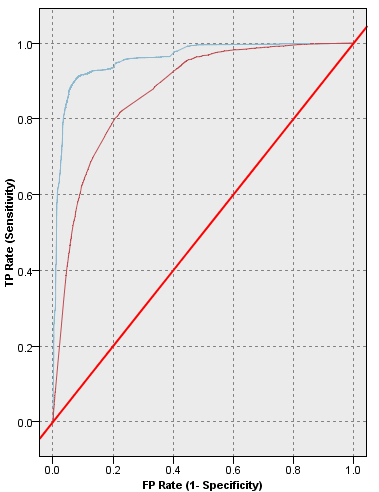
\includegraphics[scale=0.75]{ROC.PNG}
    \caption{ROC kriva za C5.0 algoritam sa i bez boosting metode}
    \label{fig:ROC}
\end{center}
\end{figure}

Nakon pravljenja modela može se videti koji atribut je u kojoj meri uticao na kasifikaciju. U ovim podacima najznačaniji atribut je PAY\_0 što predstavlja staus otplate za prethodni mesec. Odnos atributa se može videti na slici \ref{fig:najzastupljeniji}.


\begin{figure}[h!]
\begin{center}
    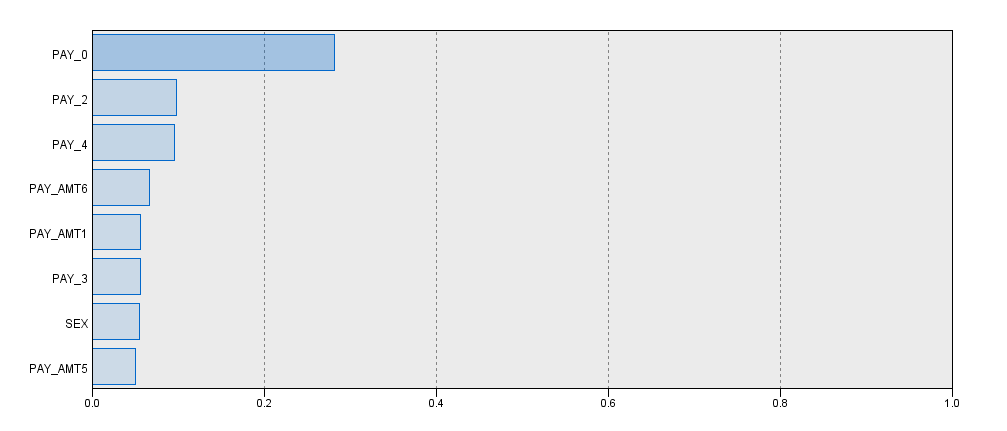
\includegraphics[scale=0.50]{Najzastuljeniji.png}
    \caption{Yastuljenost atributa u algoritmu C5.0}
    \label{fig:najzastupljeniji}
\end{center}
\end{figure}

\clearpage
\section{C\&rt}	
\label{sec:crt}


Model kod ovog algoritma je kao i kod C5.0 drvo odlučivanja, ali za razliku od njega on pravi binarno drvo. U tabelama \ref{tab:tabelaCrt}, \ref{tab:tabelaCrtBoosting} i \ref{tab:tabelaCrtBagging} su prikazane uspešnosti modela dobijenih C\&RT algoritmom bez dodtnih metoda, i sa boosting i bagging metodama.

\begin{table}[h!]
\begin{center}
\caption{C\&R tree}
\begin{tabular}{|c|l|r|c|c|} \hline
& Trening& & Test & \\ \hline
Tacni &23.051 &70.81\% &9.915 &70.58\%\\ \hline
Netacni &9.502 &29.19\% &4.133 &29.42\%\\ \hline
\end{tabular}
\label{tab:tabelaCrt}
\end{center}
\end{table}


\begin{table}[h!]
\begin{center}
\caption{C\&R tree sa korišćenjem boostin metode}
\begin{tabular}{|c|l|r|c|c|} \hline
& Trening& & Test & \\ \hline
Tacni &22.960 &70.56\% &9.835 &70.03\%\\ \hline
Netacni &9.581 &29.44\% &4.209 &29.97\%\\ \hline
\end{tabular}
\label{tab:tabelaCrtBoosting}
\end{center}
\end{table}



\begin{table}[h!]
\begin{center}
\caption{C\&R tree sa korišćenjem bagging metode}
\begin{tabular}{|c|l|r|c|c|} \hline
& Trening& & Test & \\ \hline
Tacni &22.960 &70.56\% &9.835 &70.03\%\\ \hline
Netacni &9.581 &29.44\% &4.209 &29.97\%\\ \hline
\end{tabular}
\label{tab:tabelaCrtBagging}
\end{center}
\end{table}

U tabeli \ref{tab:tabela C&RT Preciznost} možemo videi preciznost algoritma kao i meru nečistoće čvorova. Na osnovu dobijenih rezultata možemo da zaključimo da ovaj algoritam pravi lošiji model nad datim podacima.

\begin{table}[h!]
\begin{center}
\caption{Preciznost algotitma C\&RT i mera nečistoće čvorova.}
\begin{tabular}{|l|l|l|l|l|} \hline
& Trening& & Test & \\ \hline
Model &Preciznost&Gin&Preciznost&Gini\\ \hline
&0,747 &0,494 &0,755 &0,509\\ \hline
\end{tabular}
\label{tab:tabela C&RT Preciznost}
\end{center}
\end{table}
Kod ovih podataka se može pretpostaviti da je bitnije smanjiti mogućnost da se instance klase "No" klasifikuju kao instance klase "Yes". Da bi se ovo postiglo može se povećati cena tog promašaja. Nakon primene algoritma dobijaju se sledeći rezulati iz tebele \ref{tab:tabelaCrtCena} i matrica konfuzije \ref{tab:tabelaCRTKonfuzije}. Odavde dobijamo sledeće rezultste:
\begin{itemize}
    \item TPR= 0.380181 (stopa stvarno pozitvnih)
    \item TNR= 0.936788 (stopa stvarno negativnih)
    \item FPR= 0.063212 (stopa lažno pozitvnih)
    \item FNR= 0.619819 (stopa lažno negativnih)
\end{itemize}

Procenat uspesnosti modela se smanjio, ali je stopa lažno negativnih manja.
\begin{table}[h!]
\begin{center}
\caption{C\&R tree sa promenjenom cenom promašaja}
\begin{tabular}{|c|l|r|c|c|} \hline
& Trening& & Test & \\ \hline
Tacni &20.653 &65.84\% &8.859 &65.49\%\\ \hline
Netacni &10.716 &34.16\% &4.669 &34.51\%\\ \hline
\end{tabular}
\label{tab:tabelaCrtCena}
\end{center}
\end{table}

\begin{table}[h!]
\begin{center}
\caption{Matrica konfuzije za C5.0 algoritam za test skup}
\begin{tabular}{|c|l|l|l|l|} \hline
& No& Yes \\ \hline
No &TN 6.254 &FP 422 \\ \hline
Yes &FN 4.247 &TP 2.605  \\ \hline
\end{tabular}
\label{tab:tabelaCRTKonfuzije}
\end{center}
\end{table}

Algoritmi kod kojih je model drvo odlučivanja imaju pozitivnu stranu da rezultati mogu da budu lako interpretirani, odnosno nakon klasifikacije znamo zašto je instanca pripala baš toj klasi. Drvo odlučivanja koje se dobija korišćenjem C\&RT algoritma se moze videti na slici \ref{fig:CRTDrvo}.


\begin{figure}[h!]
\begin{center}
    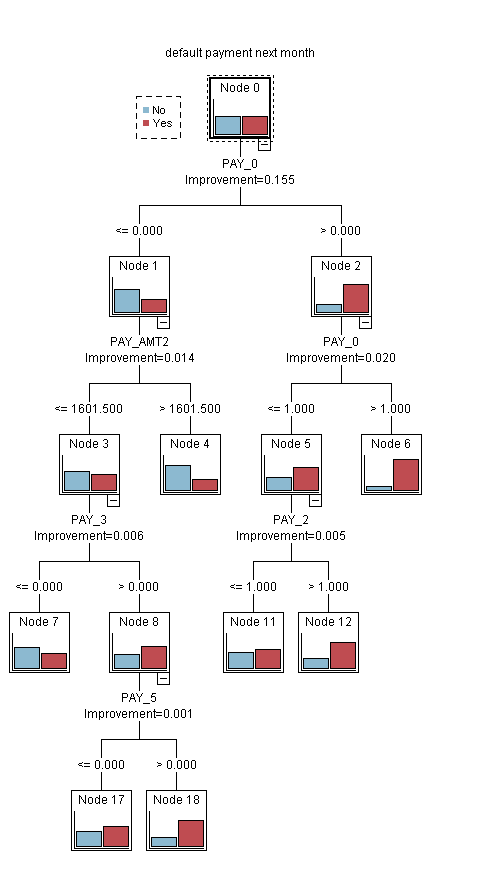
\includegraphics[scale=0.55]{crtDrvo.png}
    \caption{Drvo odlučivanja dobijeno C\&RT algoritmom}
    \label{fig:CRTDrvo}
\end{center}
\end{figure}
 

\clearpage
\section{KNN}	
\label{sec:KNN}

KNN je algoritam kod koga je klasifikacija instance zasnovana na sličnosti sa drugim
instancama. Kako se koriste mere rastojanja, potrebno je da vrednosti svih atributa budu u istom opsegu da jedan atribut ne bi vršio preveliki uticaj u odnosu na ostale. Za predprocesiranje kontinualnih atributa koristi se normalizacija, dok se kategorički atributi transformišu u binarni vektor čija je dimenzija broj različitih klasa datog atributa. Ovo predprocesiranje mozemo da obavimo sami, a ukoliko ga ne uradimo SPSS modeler će to uraditi umsto nas.
\begin{table}[h!]
\begin{center}
\caption{KNN algoritam bez dodatnih opcija.}
\begin{tabular}{|l|l|l|l|l|} \hline
& Trening& & Test & \\ \hline
Tacni &26.618 &85.85\% &11,437 &84.69\%\\ \hline
Netacni&4.691 &14.15\% &2.067 &15.31\%\\ \hline
\end{tabular}
\label{tab:tabelaKNN}
\end{center}
\end{table}


\begin{table}[h!]
\begin{center}
\caption{Preciznost algotitma KNN i mera nečistoće čvorova}
\begin{tabular}{|l|l|l|l|l|} \hline
& Trening& & Test & \\ \hline
Model &Preciznost&Gin&Preciznost&Gini\\ \hline
&0,931 &0,862&0,931&0,862\\ \hline
\end{tabular}
\label{tab:tabelaKNN Preciznost}
\end{center}
\end{table}

Pravljenje modela pomoću KNN algoritma nad podacima velikih dimenzija može da oduzme dosta vremena, zato SPSS modeler omogućava uklučivanje opcije za pravljenje modela sa redukovanim vremenom. Rezultati dobijeni primenom ove metodom se mogu videti u tebeli \ref{tab:tabelaKNNspeed}, a preciznost i mera nečistoće u \ref{tab:tabelaKNNSpeed Preciznost}.


\begin{table}[h!]
\begin{center}
\caption{KNN algoritam sa smanjenim vremenom izvršavanja.}
\begin{tabular}{|l|l|l|l|l|} \hline
& Trening& & Test & \\ \hline
Tacni &26,708 &85.3\% &11,478 &84.98\%\\ \hline
Netacni&4.604 &14.7\% &2.029 &15.02\%\\ \hline
\end{tabular}
\label{tab:tabelaKNNspeed}
\end{center}
\end{table}





\begin{table}[h!]
\begin{center}
\caption{Preciznost algotitma KNN smanjenim vremenom izvršavanja i mera nečistoćce čvorova}
\begin{tabular}{|l|l|l|l|l|} \hline
& Trening& & Test & \\ \hline
Model &Preciznost&Gin&Preciznost&Gini\\ \hline
&0,935 &0,869&0,928&0,857\\ \hline
\end{tabular}
\label{tab:tabelaKNNSpeed Preciznost}
\end{center}
\end{table}


\newpage
\section{Neuralne mreže}	
\label{sec:Neuronsle Mreze}

Neuoronske mreze daju model koji koji simulira rad nervnog sisetam. Ovaj algoritam je dobar za široku upotrebu nad podacima bez dodatnih pretpostavki. Rezultati primene algoritama bez dodatnih opcija, kao i sa boosting metodom se mogu videtu u tabelama \ref{tab:tabelaNET}, \ref{tab:tabelaNet boosting} .

\begin{table}[h!]
\begin{center}
\caption{Neuronske mreže bez dodatnih opcija.}
\begin{tabular}{|l|l|l|l|l|} \hline
& Trening& & Test & \\ \hline
Tacni &22.239 &70.8\% &9,535 &70.39\%\\ \hline
Netacni&9,172 &29,2\% &4,011 &29,61\%\\ \hline
\end{tabular}
\label{tab:tabelaNET}
\end{center}
\end{table}


\begin{table}[h!]
\begin{center}
\caption{Neuronske mreže bez dodatnih opcija. Preciznost i Gini}
\begin{tabular}{|l|l|l|l|l|} \hline
& Trening& & Test & \\ \hline
Model &Preciznost&Gin&Preciznost&Gini\\ \hline
&0,789 &0,578&0,789&0,577\\ \hline
\end{tabular}
\label{tab:tabelaNET Preciznost}
\end{center}
\end{table}

\begin{table}[h!]
\begin{center}
\caption{Neuronske mreže sa korišćenjem boosting metode.}
\begin{tabular}{|l|l|l|l|l|} \hline
& Trening& & Test & \\ \hline
Tacni &22.501 &71.73\% &9,706 &71.76\%\\ \hline
Netacni&8.866 &28.27\% &3,819 &28.24\%\\ \hline
\end{tabular}
\label{tab:tabelaNet boosting}
\end{center}
\end{table}

\begin{table}[h!]
\begin{center}
\caption{Neuronske mreže sa korišćenjem boosting metode. Preciznost i Gini}
\begin{tabular}{|l|l|l|l|l|} \hline
& Trening& & Test & \\ \hline
Model &Preciznost&Gin&Preciznost&Gini\\ \hline
&0,789 &0,578&0,789&0,577\\ \hline
\end{tabular}
\label{tab:tabelaNETboosting Preciznost}
\end{center}
\end{table}









\section{Zaključak}
\label{sec:zakljucak}

Cilj istraživanja je bio da se napravi model za klasifikaciju klijenata banke na osnovu toga da li će izmiriti svoje obaveze za sledeci mesec. U istraživanju je korišćeno nekoliko različitih načina za predprocesiranje i algoritama za pravljenje modela. 

Ispitani algoritmi su C5.0 i C\&RT koji prave drvo odlučivanja, KNN koji poredi sličnost sa ostalim instancama i neuronske mreže. Na osnovu svih ispitanih rezultata može se zaklučiti da C5.0 algoritam sa boosting metodom daje najbolje rezultate, dok nam C\&RT algoritam daje najjednostavniji model. 



\end{document}







